\documentclass[a4paper,11pt]{article}
\usepackage[latin1]{inputenc}
\usepackage[T1]{fontenc}
\usepackage{amsmath}
\usepackage{a4wide}
\usepackage{booktabs}
\usepackage{graphicx}

\title{Genomics and Bioinformatics}
\date{October 30, 2012}
\author{Examination - Week 7}
\begin{document}
\maketitle

\section*{Question 1 - Sequence Alignment}

\subsection*{Linear gap penalty}
Using the following scoring: a match is worth 2 points, a mismatch is penalized -1,
and a gap is penalized -2 points, find all optimal 
alignments of the sequences\\
\texttt{ATTCCGTTA}, \texttt{ATCGA}\\
by the Needleman-Wunsch algorithm.  


\subsection*{Affine gap penalty}

Calculate the scores of the previous alignments using a gap opening
penalty of -2 points and a gap extension penalty of -1. 
Are the previous alignments still equivalent?

\section*{Question 2 - Phylogenetic trees}

The \textit{INS} gene (insulin peptide precursor) is shared among many vertebrates.

The table below provides BLAST scores of pairwise
alignments for six \textit{INS} family proteins from four different species, 

\begin{enumerate}
\item {\bf hs\_ins} from {\it Homo sapiens}, i.e. human,
\item {\bf xt\_ins} from {\it Xenopus tropicalis}, i.e. frog,
\item {\bf rn\_ins1} and {\bf rn\_ins2} from {\it Rattus norvegicus}, i.e. rat,
\item {\bf mm\_ins1} and  {\bf mm\_ins2} from {\it Mus musculus}, i.e. mouse.
\end{enumerate}

\begin{center}
	\begin{tabular} {| l || l | l | l | l | l | l |}
	\hline
 	                    & hs\_ins & xt\_ins & rn\_ins1 & rn\_ins2 & mm\_ins1 & mm\_ins2 \\ \hline\hline
	hs\_ins        & -            & 414             &  499         & 612       & 589           & 421 \\	\hline
	xt\_ins      & 444       & -                  &  111        & 125       & 221           & 91 \\	\hline
	rn\_ins1       & 546      & 178              & -             & 667       & 976           & 690 \\	\hline
	rn\_ins2       & 411      & 129              & 800        & -            & 702           & 899 \\	\hline
	mm\_ins1    & 466      & 241              & 1112      & 680       & -                & 630 \\ 	\hline
	mm\_ins2    & 666      & 113              & 800        & 932       & 780           & - \\
	\hline
	\end{tabular}
\end{center}
\vspace{0.05 cm}

\begin{enumerate}
\item Based on the table above, draw the gene tree for the six \textit{INS}
  proteins ({\bf mm\_ins1}, {\bf mm\_ins2}, {\bf rn\_ins1} and {\bf rn\_ins2}, {\bf xt\_ins}, {\bf hs\_ins}). 
  Indicate speciation and duplication events on the graph.
\item Using this tree, give examples of:
  \begin{itemize} 
  \item an orthologous pair, 
  \item a paralogous pair in the same species, and 
  \item a paralogous pair in different species.
  \end{itemize}
\end{enumerate}


\section*{Question 3 - Genome Assembly}

Consider the following reads:
TGCATGC, CCATGCA, CCATGTC, ATGCCAT

\begin{enumerate}
\item Construct the overlap graph based on the above reads, using an
  overlap size of $4$ bases.
  Draw a path that goes
  through every \emph{vertex} (Hamiltonian path), and write the
  corresponding contig. 
\item Make a list $S_4$ of all unique $4$-mers (9 elements) and the
  list $S_5$ of all (non-unique) 5-mers (12 elements). 
\item Construct the De Bruijn graph with $S_4$ as vertex set and
  $S_5$ as edge set.
\item Add one edge to make this graph Eulerian and find two Eulerian paths.
  Write down the corresponding contigs and indicate which of them is
  compatible with the full reads.
\end{enumerate}


\section*{Question 4 - Hidden Markov Model}

%\subsection*{The Viterbi algorithm}
%\noindent
Consider the Hidden Markov Model represented in the figure below. The
hidden states are $S$, $X$ and $Y$, with emitted symbols 
$-$, $A$, $C$, $G$ and $T$. The non-zero emission probabilities are
specified under the
corresponding hidden states. 

%\begin{center}
%\vskip -4.5cm
%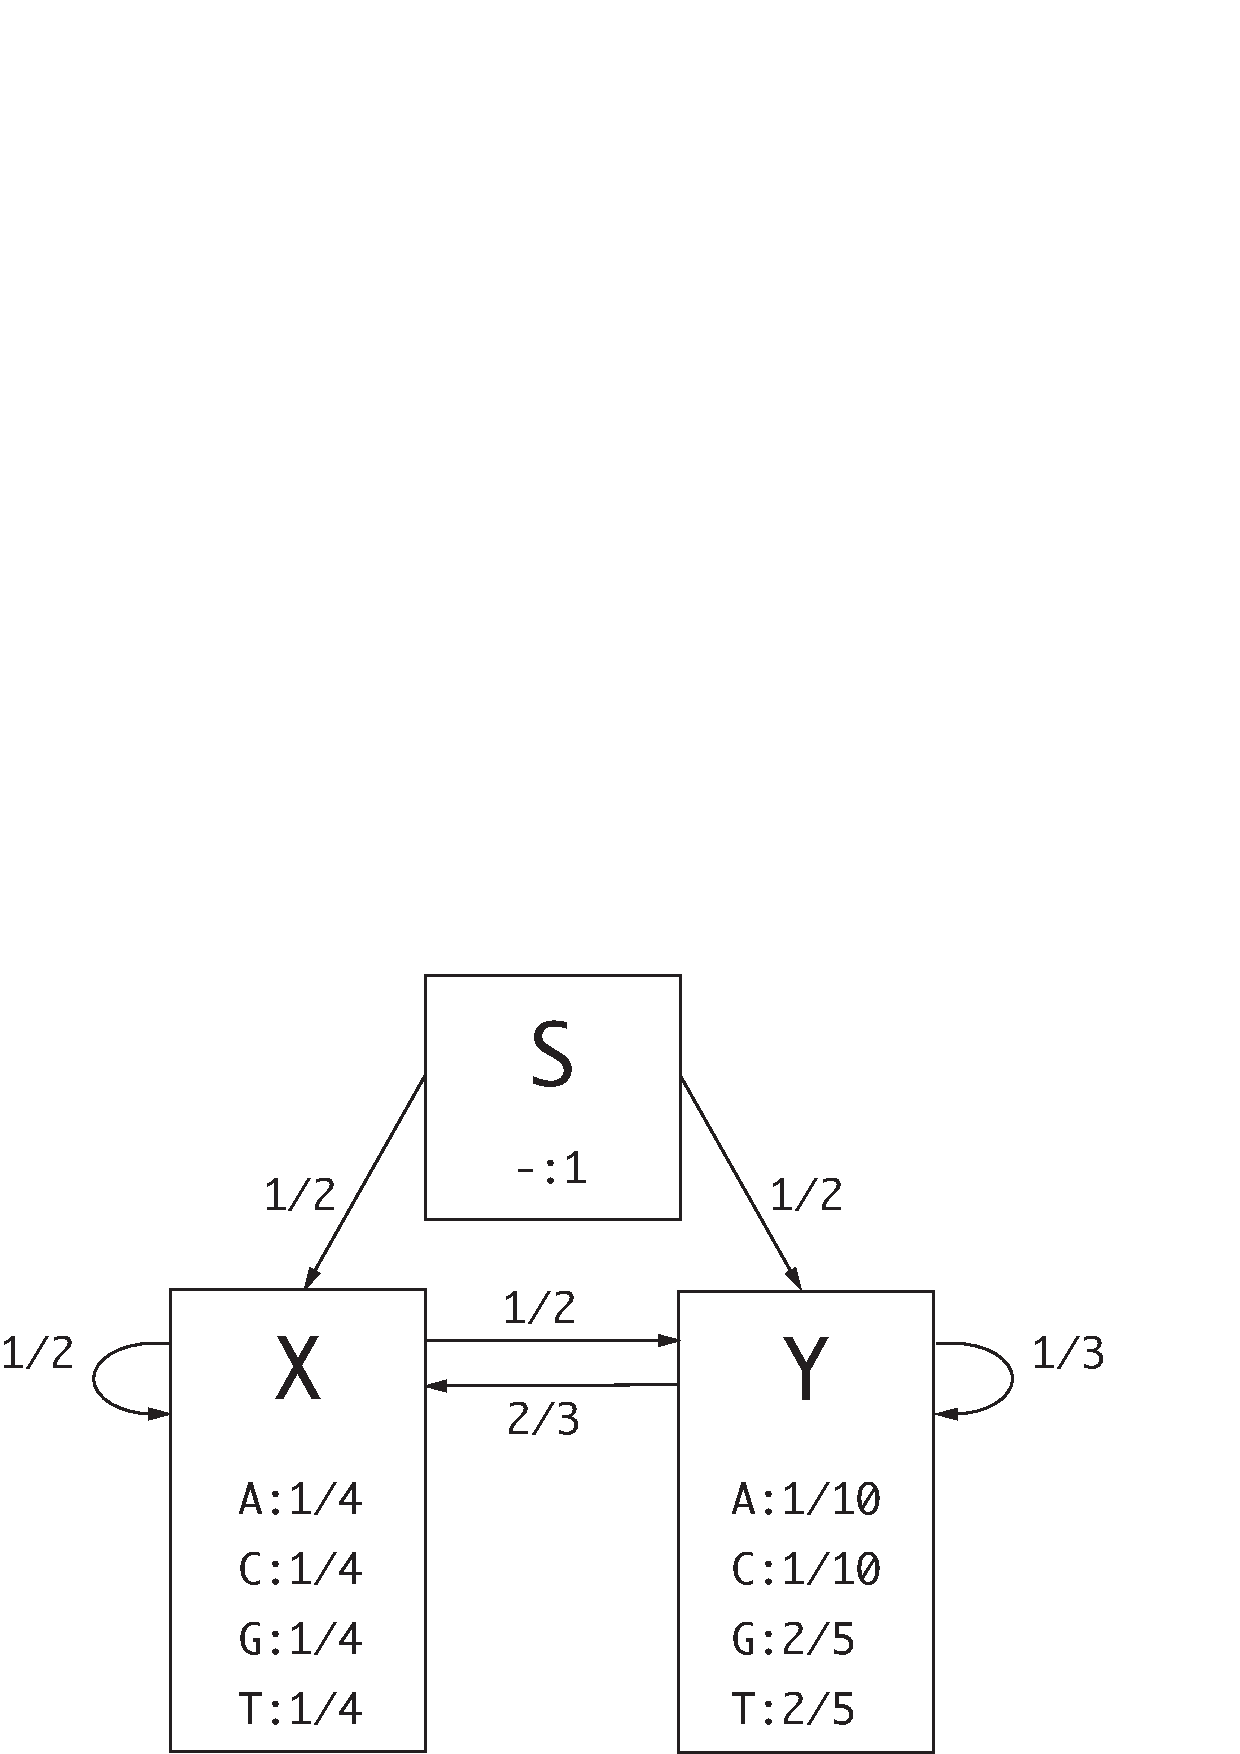
\includegraphics[width=0.4\textwidth]{fig1.pdf}\\
%\end{center}

%The Viterbi algorithm is based on the following scoring function:
%$$
%F_{n,s} = E(T_n, s) \cdot \max_{\sigma \in \{S, X, Y\}}\left\{F_{n-1,
%  \sigma} \cdot M(\sigma, s)  \right\}~, \ n = 1, 2, \dots~, 
%$$
%where the initial condition is $F_{0, \sigma} = 1$ if $\sigma = S$ and
%$F_{0, \sigma} = 0$ otherwise. Here $n$, $T_n$ and $s$ correspond to
%the column number, symbol in column $n$ and hidden state in the table,
%respectively, and $E$ and $M$ are the emission and transition
%matrices.  

Use the Viterbi algorithm to fill the scoring table and then use
backtracking to find the most probable hidden state sequence
associated with the observed sequence "CGA": 

\begin{center}
\vskip -5cm
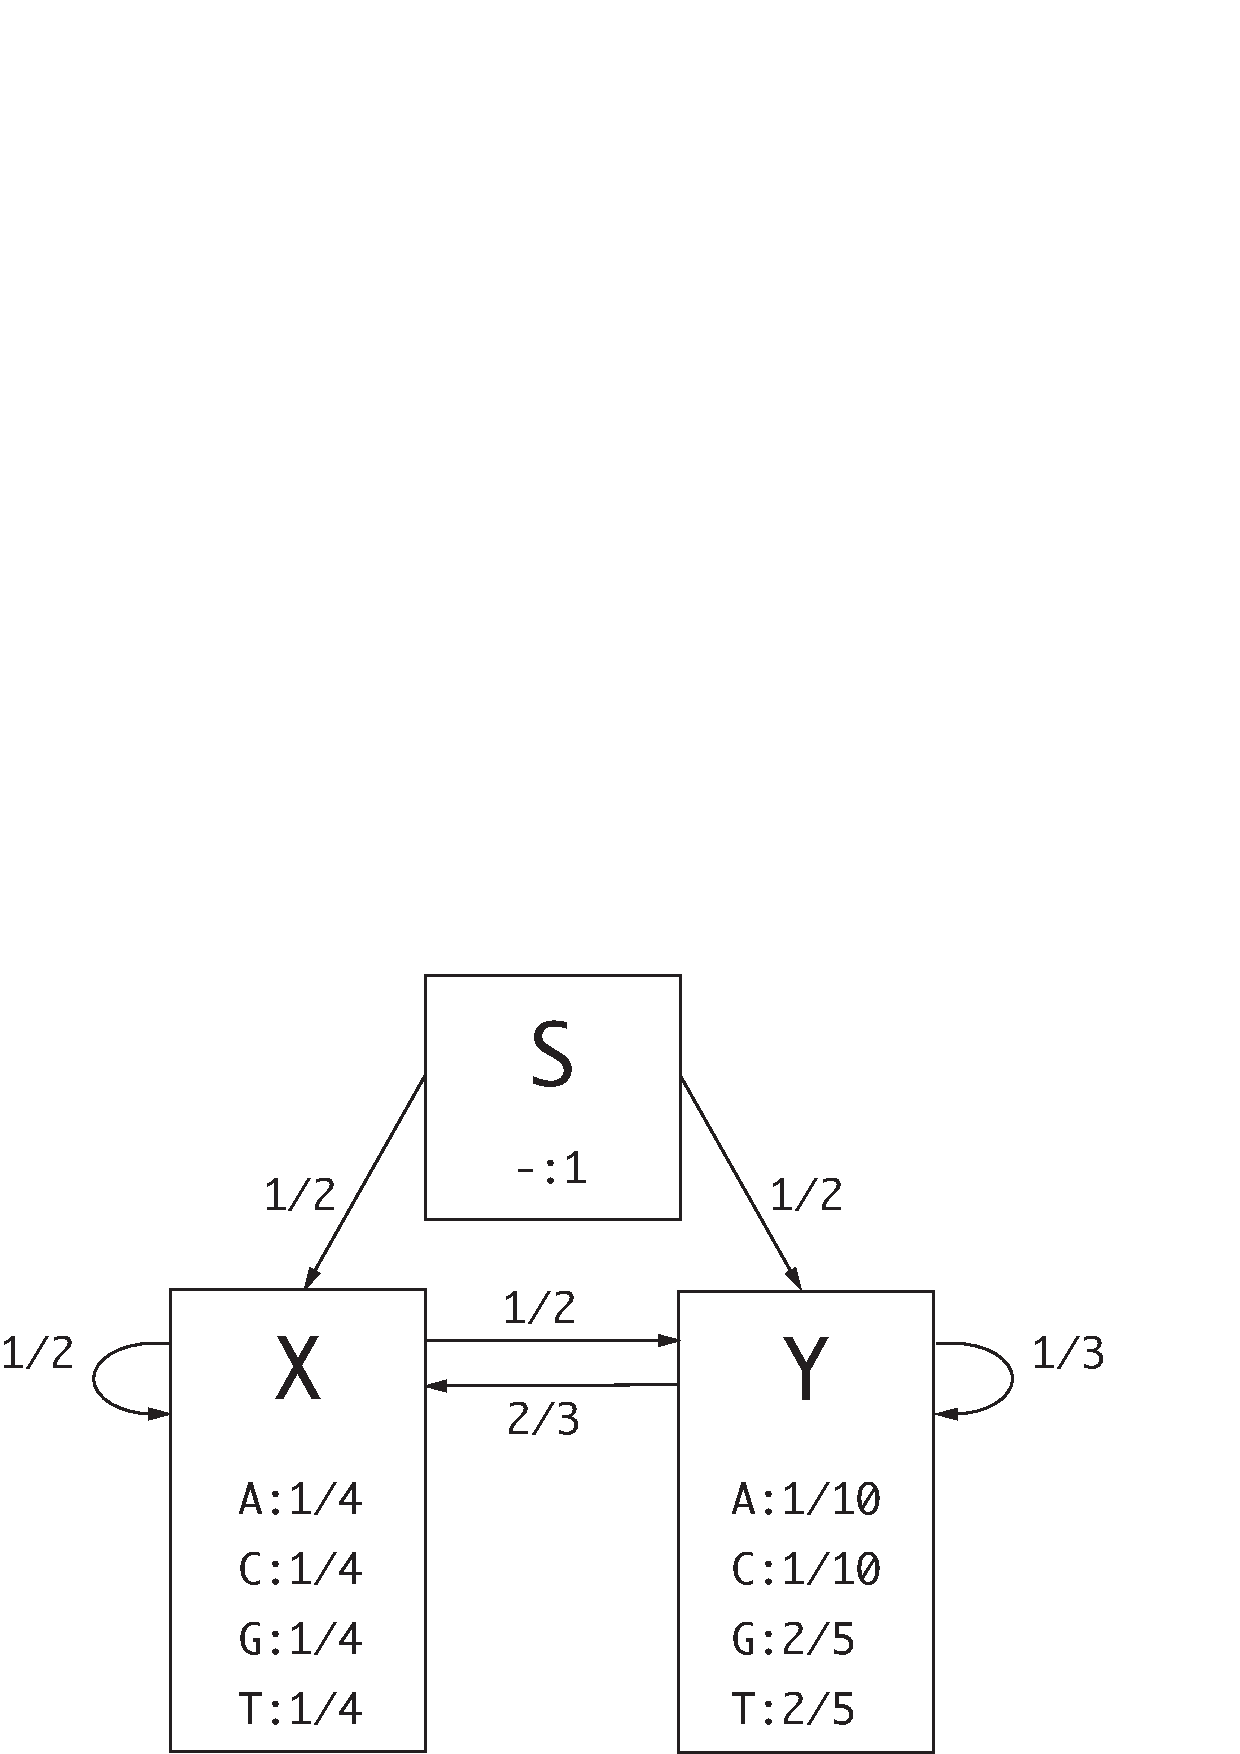
\includegraphics[width=0.4\textwidth]{fig1.pdf}
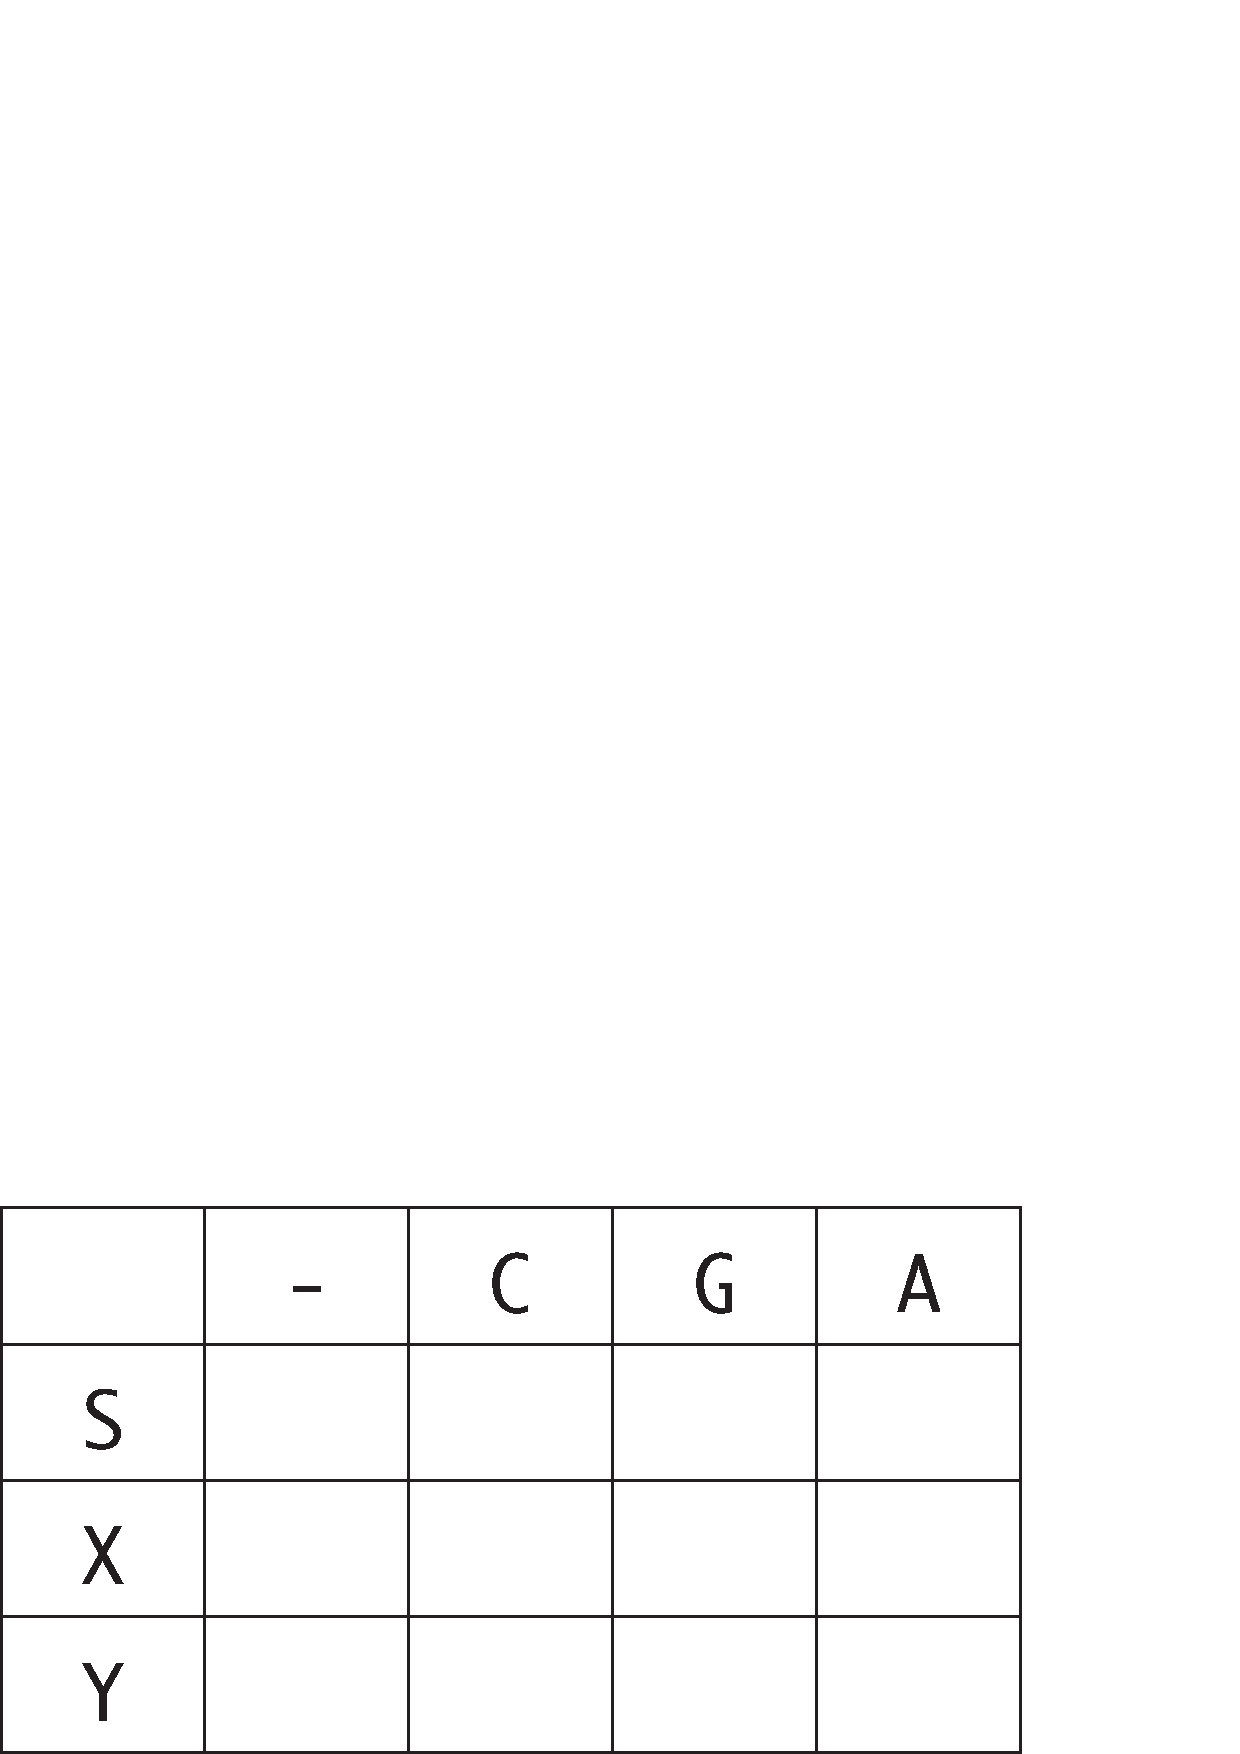
\includegraphics[width=0.5\textwidth]{fig2.pdf}
\end{center}

\end{document}
